\documentclass[11pt,a4paper]{article}

% --- FONT + LANGUAGE ---
\usepackage{fontspec} % for custom fonts (requires xelatex/lualatex)
\setmainfont{Kalam} % <-- requires Kalam installed

% --- MATH PACKAGES ---
\usepackage{amsmath,amssymb,amsthm}
\usepackage{mathtools}
\usepackage{physics}   % nice shorthand like \dv, \pdv
\usepackage{bm}        % bold math
\usepackage{accents}
\usepackage{float}
\usepackage{graphicx}
\usepackage{comment}
% --- PAGE & STYLE ---
\usepackage[a4paper,margin=1in]{geometry}
\usepackage{titlesec} % custom section titles
\usepackage{fancyhdr} % headers/footers
\usepackage{xcolor}   % colors

% --- HEADER / FOOTER ---
\pagestyle{fancy}
\fancyhf{}
\lhead{\textbf{Course Summary}}
\rhead{\leftmark}
\cfoot{\thepage}

% --- THEOREM ENVIRONMENTS ---
\newtheorem{theorem}{Theorem}[section]
\newtheorem{lemma}[theorem]{Lemma}
\newtheorem*{definition}{Definition}
\newtheorem{example}[theorem]{Example}
\newtheorem*{exercise}{Exercise}
\newtheorem{proposition}[theorem]{Proposition}
\newtheorem{corollary}[theorem]{Corollary}

% --- CUSTOM MACROS ---
\newcommand{\lecture}[2]{
	\section*{Lecture #1 -- #2}
	\addcontentsline{toc}{section}{Lecture #1: #2}
}
\newcommand{\solution}[1]{
	\subsection*{Solution}
	#1
}
\newcommand{\problems}[1]{
	\subsection*{Problems}
	#1
}
\graphicspath{{figures/}}

% --- DOCUMENT ---
\begin{document}
	
	\begin{center}
		{\Huge \textbf{Course Summary}} \\[1em]
		{\Large Advanced Mathematical Physics I (Equations of Physics)} \\[0.5em]
		{\large Andrew Moyer} \\[2em]
	\end{center}
	
	\tableofcontents
	\newpage
	
	% --- SAMPLE CONTENT ---
	\lecture{1}{Introduction to Equations of Mathematical Physics}
	% Canonical Linear PDEs in Mathematical Physics
	% Each equation is annotated with its main physical meaning.
	
\textbf{Elliptic (equilibrium / static):}
\begin{align*}
	\text{Laplace:}\quad & \Delta u = 0, \\[6pt]
	\text{Poisson:}\quad & \Delta u = f(x), \\[6pt]
	\text{Helmholtz:}\quad & \Delta u + k^2 u = 0.
\end{align*}

\textbf{Parabolic (diffusion / smoothing):}
\begin{align*}
	\text{Heat / Diffusion:}\quad & u_t = \kappa \Delta u, \\[6pt]
	\text{Schrödinger (free):}\quad & i \hbar u_t = -\tfrac{\hbar^2}{2m} \Delta u.
\end{align*}

\textbf{Hyperbolic (wave propagation):}
\begin{align*}
	\text{Wave:}\quad & u_{tt} = c^2 \Delta u, \\[6pt]
	\text{Klein--Gordon:}\quad & u_{tt} - c^2 \Delta u + m^2 u = 0.
\end{align*}

	These are the equations of mathematical physics that we will study. They are all similar as they are linear differential operators actingo on an unknonw function $u$. We will frequently use this fact to find solutions. Because the equations are linear, a sum of solutions is also a solution.
	\newline
	
	Pavel derives most of these equations by defining forces and interactions on a lattice, then taking a continuum limit. This seems to be an important skill of a physicist as it reflects a deeper understanding of the equations. From the lattice standpoint, we can see an interesting feature of emergence in these equations. Symmetry is broken at the micoroscopic level but reappears at the macroscopic level.

\begin{align*}
	\partial_t \vec{u} + (\vec{u}\!\cdot\!\vec{\nabla})\,\vec{u}
	&= -\,\frac{1}{\rho}\,\vec{\nabla} p, \\[6pt]
	\partial_t \rho + \vec{\nabla}\!\cdot(\rho \vec{u})
	&= 0.
\end{align*}


\begin{align*}
	\partial_{t}\rho+\vec{\nabla}(\rho\vec{u})=0
\end{align*}
These are the navier stokes equations. the nonlinearity in equation (8) causes most of the difficulty in solving the equation. Interestingly, Pavel says that these equations cannot be derived from a discrete lattice model. These linear PDEs often appear as approximations to more complicated nonlinear problems.
\problems{
\begin{exercise}
Show that the $(2+1)$ wave equation 
$$
u_{yy} +u_{xx} - u_{tt} = 0
$$
has rotational invariance
\begin{align*}
	\begin{bmatrix}
		x \\[6pt]
		y
	\end{bmatrix}
	\mapsto
	\begin{bmatrix}
		\cos\theta & \sin\theta \\[6pt]
		-\sin\theta & \cos\theta
	\end{bmatrix}
	\begin{bmatrix}
		x \\[6pt]
		y
	\end{bmatrix}.
\end{align*}
and Lorentz invariance
\begin{align*}
	\begin{bmatrix}
		t \\[6pt]
		x
	\end{bmatrix}
	\mapsto
	\begin{bmatrix}
		\cosh\theta & \sinh\theta \\[6pt]
		\sinh\theta & \cosh\theta
	\end{bmatrix}
	\begin{bmatrix}
		t \\[6pt]
		x
	\end{bmatrix},
\end{align*}
 \end{exercise}
 \solution{
 We have $u(x,y)\to u(x^{\prime},y^{\prime})$
 where
 $$
 x^{\prime}(x,y) = \cos\theta x + \sin\theta y
 $$
$$
y^{\prime}(x,y) = -\sin\theta x +\cos\theta y
$$
 }
so we must change the operators.
$$
\frac{\partial}{\partial x} = \frac{\partial x^{\prime}}{\partial x}\frac{\partial}{\partial x^{\prime}} + \frac{\partial y^{\prime}}{\partial x}\frac{\partial}{\partial y^{\prime}} = \cos\theta\partial_{x^{\prime}} -\sin\theta\partial_{y^{\prime}}
$$
$$
\frac{\partial}{\partial y} = \frac{\partial x^{\prime}}{\partial y}\frac{\partial}{\partial x^{\prime}} + \frac{\partial y^{\prime}}{\partial y}\frac{\partial}{\partial y^{\prime}} = \sin\theta\partial_{x^{\prime}}+\cos\theta\partial_{y^{\prime}}
$$
}
If we square both operators we will see that the cross terms cancel and use the identity $\sin^{2}\theta+\cos^{2}\theta = 1$ to get
$$
u_{y^{\prime}y^{\prime}}(x^{\prime},y^{\prime}) + u_{x^{\prime}x^{\prime}}(x^{\prime},y^{\prime}) - u_{tt}(x^{\prime},y^{\prime}) = 0
$$
So we see that solutions to the wave equation in $(2+1)$ dimensions have rotational symmetry. For the Lorentz transform we repeat the same process except we use the analagous hyperbolic trig identitity $\sinh^{2}\theta-\cosh^{2}\theta = 1$ to get
$\sin^{2}\theta+\cos^{2}\theta = 1$ to get
$$
u_{yy}(x^{\prime},y^{\prime}) + u_{x^{\prime}x^{\prime}}(x^{\prime},y^{\prime}) - u_{t^{\prime}t^{\prime}}(x^{\prime},y^{\prime}) = 0
$$
so we also see that waves are lorentz invariant as well, there is no preferred frame of reference.
	\lecture{2}{Canonical Forms of Mathematical Equations and Beginning of Wave Equation Solution}
	Consider the following equation
	\begin{align}
		\sum_{i,j=1,...,n}B^{ij}\frac{\partial}{\partial x^{i}}\frac{\partial}{\partial x^{j}}u+\sum_{i=1,...,n}A^{i}\frac{\partial}{\partial x^{i}}u + cu = 0
		\end{align}.
		where the coefficients are constant. We would like to study how these equations chane under the change of variables
		$$
		\tilde{x}^{i} = \tilde{x}^{i}(x^{1},...,x^{n})
		$$.
		We arealso interested in the transformation
		$$
		\tilde{u} = ue^{-f(x^{1},...,x^{n})}
		$$
		Before we derive the explicit transformation we review the algebra of differential operators, which must be preserved under the coordinate transformation. Say we have $f\in C^{\infty}(\mathbb{R}^{n})$ and a set of generators $\partial_{1},...,\partial_{n}$. Acting on our test function $\phi(\vec{x})$ we have
		$$
		(\partial_{i}f(\vec{x}))\phi(\vec{x}) =  \frac{\partial f(\vec{x})}{\partial x^{i}}\phi(\vec{x})+f(\vec{x})\frac{\partial\phi(\vec{x})}{\partial x^{i}} = [\frac{\partial f(\vec{x})}{\partial x^{i}}+f(\vec{x})\frac{\partial}{\partial x^{i}}]\phi(\vec{x})
		$$
		So the we conclude that
		$$
		\partial_{i}f(\vec{x}) =  (\partial_{i}f)(\vec{x})+f(\vec{x})\partial_{i}
		$$
		From this we can find the following commutator is
		$$
		[\partial_{i},f(\vec{x})] = (\partial_{i}f)(\vec{x})
		$$ 
		We can also conjugate the differential operator $\partial_{i}$ and find
		$$
		e^{-f(\vec{x})}\partial_{i}e^{f(\vec{x})} = \partial_{i}+(\partial_{i}f)(\vec{x})
		$$
		If $f(\vec{x}) = x^{j}$ then we have the \textit{Weyl Algebra}
\begin{align}
[\partial_{i},x^{j}]=\delta_{i}^{j}
\end{align}
Now that we have our algebra we would like to study and invertible linear transformation
$$
x^{i}= T^{i}_{\ j}\tilde{x}^{j}
$$
and
$$
\partial_{i}=\hat{T}_{i}^{\ j}\tilde{\partial}_{j} \Leftrightarrow \vec{\nabla} = T^{-1}\tilde{\vec{\nabla}}\cdot 
$$
We know that the algebra
$$
[\tilde{\partial}_{j},\tilde{x}^{i}]=\delta^{i}_{j}
$$
must be preserved.
If we substitute in our new variables we can easily calculate
$$
(\hat{T}T)^{i}_{j} = \delta^{i}_{j}\Rightarrow \hat{T} = T^{-1}
$$
So whatever linear transformation we choose for the variables, the linear transformation for the derivative operators must be the inverse. From this we also conclude the transformation
\[
\partial_i=\hat{T}_i{}^{\,j}\,\tilde{\partial}_j
\qquad\Longleftrightarrow\qquad
\vec{\nabla}=\vec{\tilde{\nabla}}\,T^{-1}.
\]
If we consider a general linear transformation $f(\vec{x}) = (\vec{\alpha},\vec{x})$ Then we have the conjugation
$$
e^{(\vec{\alpha},\vec{x})}\partial_{i}e^{(\vec{\alpha},\vec{x})} = \partial_{i} + \alpha_{i}\Leftrightarrow e^{(\vec{\alpha},\vec{x})}\vec{\nabla}e^{(\vec{\alpha},\vec{x})} = \vec{\nabla} +\vec{\alpha}
$$
Let us use these tools to study the generic differential operator
$$
D = (\vec{\nabla},B\vec{\nabla}) + (\vec{A},\vec{\nabla}) +C
$$
and use a result from the study of quadratic forms that $B$ can always be transformed in the following way. We now what to find the transformation $x^{i} = T^{i}_{\ j}\tilde{x}^{j}$ such that we get $B$ into a canoncial form
\[
\tilde{B}_{n,p,q} =
\begin{pmatrix}
	I_p & 0 & 0 \\
	0 & -I_q & 0 \\
	0 & 0 & 0_{\,n-p-q}
\end{pmatrix},
\]
We need to find $\vec{\alpha}$ in the following transformation of the operator
\begin{align}
\tilde{D} = e^{-(\vec{\alpha},\vec{x})}De^{(\vec{\alpha},\vec{x})}
\end{align}
We will use the following trick
$$
e^{-(\vec{\alpha},\vec{x})}\partial_{i}\partial_{j}e^{(\vec{\alpha},\vec{x})} = e^{-(\vec{\alpha},\vec{x})}\partial_{i}e^{(\vec{\alpha},\vec{x})}e^{-(\vec{\alpha},\vec{x})}\partial_{j}e^{(\vec{\alpha},\vec{x})} = (\partial_{i}+\alpha_{i})(\partial_{j}+\alpha_{j})
$$
The conjugation shifts the partial derivatives by a constant. Appying this to $D$ gives us
\begin{align}
	\scriptstyle{ \tilde{D} = (\vec{\nabla}+\vec{\alpha}, \tilde{B}(\vec{\nabla}+\vec{\alpha})) + (\tilde{\vec{A}},(\vec{\nabla}+\vec{\alpha})) + C =  (\vec{\nabla},\tilde{B}\vec{\nabla})
	+ \underline{2(\vec{\nabla},\tilde{B}\vec{\alpha})}
	+ (\vec{\alpha},\tilde{B}\vec{\alpha})
	+ \underline{(\tilde{\vec{A}},\vec{\nabla})}
	+ (\tilde{\vec{A}},\vec{\alpha})
	+ C}
\end{align}
We would like to choose the transformation such that the underlined terms simplify as much as possible to return to the canonical forms of lecture 1.
We have
$$
2\tilde{B}\vec{\alpha} + \tilde{A} =2 \cdot
\operatorname{diag}\!\left(
\underbrace{1,\dots,1}_{p},\,
\underbrace{-1,\dots,-1}_{q},\,
\underbrace{0,\dots,0}_{n-p-q}
\right)
\begin{bmatrix}
	\alpha_1 \\
	\alpha_2 \\
	\vdots \\
	\alpha_n
\end{bmatrix}
+
\begin{bmatrix}
	\tilde{A}_{1} \\
	\tilde{A}_{2} \\
	\vdots \\
\tilde{A}_{n}
\end{bmatrix} = \begin{bmatrix}
0 \\
\vdots \\
0\\
\tilde{A}_{p+q+1}\\
\vdots\\
\tilde{A}_{n}
\end{bmatrix} \equiv \tilde{A}^{*}
$$
We can choose the first $p+q$ components of $\alpha$ to cancel the first $p+q$ components in $\tilde{\vec{A}}$. We have $\alpha_{i} = -\frac{\tilde{A}_{i}}{2}$ for the first $p$ components and $\alpha_{j} = \frac{\tilde{A}_{j}}{2}$ for the next $q$ components. We have the following cases:
\begin{itemize}
\item $p+q = n$: $\tilde{D} = \tilde{\partial}_{1}^{2}+...+\tilde{\partial}_{p}^{1}-\tilde{\partial}_{p+1}^{2}-...-\tilde{\partial}_{q}^{2}+\tilde{C} =  0$ with $\tilde{C} = 0$ or positive or negative.
\begin{itemize}
\item For $\tilde{C} = 0$ we get the wave equation in signature $(p,q)$
\item $q = 0$ is Laplace equation
\item $q = 0$ is normal wave equation
\end{itemize} 
For $\tilde{C}\neq 0$
\begin{itemize}
\item $\tilde{C}>0$ we can do another rescaling of coordinates to $\tilde{x}_{i}\to\frac{\tilde{x}_{i}}{\sqrt{\tilde{C}}}$ to get the Klein gordon equation
\end{itemize}
\item $p+q < n$ 
$$
\tilde{A}^{*} \to \begin{bmatrix}
	0 \\
	\vdots \\
	0\\
	1\\
	0\\
	\vdots\\
	0
\end{bmatrix}
$$ we get $\tilde{D} =  \tilde{\partial}_{1}^{2}+...+\tilde{\partial}_{p}^{2}-\tilde{\partial}_{p+1}^{2}-...-\tilde{\partial}_{p+q}^{2} + \tilde{\partial}_{p+q+1} + \tilde{C}$ . We use our conjugation result from earlier to get $\tilde{\partial}_{p+q+1} + \tilde{C} = e^{-\tilde{C}\tilde{x}_{p+q+1}}\tilde{\partial}_{p+q+1}e^{\tilde{C}\tilde{x}_{p+q+1}} $ to get the canoncial form
$$
\tilde{D}^{} =  \tilde{\partial}_{1}^{2}+...+\tilde{\partial}_{p}^{2}-\tilde{\partial}_{p+1}^{2}-...-\tilde{\partial}_{p+q}^{2} + \tilde{\partial}_{p+q+1}$$ which acts a heat or diffusion like operator.
\end{itemize}
Now for an example. Consider
$$
u_{xx} +2u_{xy}-3u_{yy} = 0
$$
We can rewrite the operator  as
$$
[(\partial_{x}+\partial_{y})^{2}-\partial_{y}^{2}] - 3\partial_{y}^{2} = (\partial_{x}+\partial_{y})^{2}-2\partial_{y}^{2}
$$
From this form we see that $\partial_{\tilde{x}} = \partial_{x}+\partial_{y}$ and $\partial_{\tilde{y}}^{2}=2\partial_{y}^{2}$. From these relations we deduce the following four equations
\begin{itemize}
\item $(\partial_{x}+\partial_{y})\tilde{y} = 0$
\item $\partial_{y}\tilde{x} = 0 $
\item $(\partial_{x}+\partial_{y})\tilde{x} = 1$
\item $2\partial_{y}\tilde{y} = 1 $
\end{itemize}
We can easily conclude the appropriate change of variables is $\tilde{x}=x$ and $\tilde{y}=\frac{1}{2}(y-x)$.
We can rewrite the orginial equation as
$$
(\partial_{x}+3\partial_{y})(\partial_{x}-\partial{y})u = 0 \Leftrightarrow \partial_{\xi}\partial_{\eta}u = 0
$$
This form can be solved easily. We conclude $\partial_{\eta}u = f(\eta)$. We can also conclude $u(\eta,\xi) = g(\eta)+h(\xi)$. Playing the same game as earlier we can conlcude
$$
u(x,y) =  g(\frac{3}{4}x-\frac{1}{4}y)+h(\frac{1}{4}y+\frac{1}{4}x)
$$
\problems{
	\begin{exercise}
		Find the normal form of the equation
		\[
		u_{xx} + 2u_{xy} + u_{yy} + u_{x} + u = 0.
		\]
	\end{exercise}
	\solution{We notice the differential operator is $(\partial_{x}+\partial_{y})^{2}\equiv \partial_{\tilde{y}}^{2}$ and likewise we define $\partial_{x}\equiv \partial_{\tilde{x}}$. Now we can solve
\begin{itemize}
\item $(\partial_{x}+\partial_{y})\tilde{y} = 1$
\item $(\partial_{x}+\partial_{y})\tilde{x} = 0$
\item $\partial_{x}\tilde{x} = 1$
\item $\partial_{x}\tilde{y} = 0$
\end{itemize}
We easily find that $\tilde{x} =  x - y$ and $\tilde{y} =y$. This gives us $\partial_{x} = \partial_{\tilde{x}}$ and $\partial_{y} = \partial_{\tilde{y}}-\partial_{\tilde{x}}$. Then we get
$$
u_{\tilde{y}\tilde{y}} + u_{\tilde{x}} + u = 0
$$

We can introduce a new variable to solve for $u(\tilde{x},\tilde{y}) = e^{a\tilde{x}}v(\tilde{x},\tilde{y})$. Doing the substitution we get
$$
e^{a\tilde{x}}v(\tilde{x},\tilde{y})+e^{a\tilde{x}}v(\tilde{x},\tilde{y})+e^{a\tilde{x}}(a+1)
$$
Choosing $a = -1$ gives us the heat equation
$$
v_{\tilde{y}\tilde{y}} + v_{\tilde{x}} = 0
$$
}
	\begin{exercise}
		Find the normal form of the equation
		\[
		u_{xx} + 2u_{xy} + u_{yy} - u_{zz} = 0.
		\]
		Write its general solution.
	\end{exercise}
		}
		\solution{
		We notice the perfect square operator $(\partial_{x}+\partial_{y})^{2}\equiv \partial_{\xi}$. But we need another variable $\eta(x,y)$. We see operator has the form
		$$
	(\partial_{x},\partial{y})
	\begin{pmatrix}
			1 & 1 \\
			1 & 1
\end{pmatrix}
\begin{pmatrix}
\partial_{x} \\
\partial{y}			
\end{pmatrix}
		$$
	We solve for the eigenvectors $(1,1)$ and $(1,-1)$. So we find that $\eta(x,y)=x-y$ The equation is now the wave equation
	$$
	u_{\xi\xi}(\xi,\eta,z) - u_{zz}(\xi,\eta,z) = 0
	$$ We only have the general solution for $1+1$ dimensions in class. We know have a 3rd variable for $2+1$ but this 3rd coordinate is independent of the other two. The general solution is
$$	
	u(\xi,\eta,z) = F(\xi+z,\eta)+G(\xi-z,\eta)
$$
	
		}
	
		\begin{exercise}
			Find the  canonical form of
			$$17\,\frac{\partial^2 u}{\partial x^2}
			+ 20\,\frac{\partial^2 u}{\partial x \partial y}
			+ 8\,\frac{\partial^2 u}{\partial y^2}
			+ 8\,\frac{\partial^2 u}{\partial x \partial z}
			+ 4\,\frac{\partial^2 u}{\partial y \partial z}
			+ \frac{\partial^2 u}{\partial z^2}
			+ \frac{\partial u}{\partial x}
			+ u = 0$$
		\end{exercise}

\solution{
We first note that
\[
B =
\begin{bmatrix}
	17 & 10 & 4 \\
	10 & 8 & 2 \\
	4 & 2 & 1
\end{bmatrix}
\]
We split the mixed terms in half because the matrix is symmetric. If we diaganolize we must find the eigenvalues. We have $\lambda_{\pm} = 13 \pm 8\sqrt{2}$ which are both greater than 0. And the 3rd eigenvalue is 0. So $p = 2$, $q = 0$ and $n-p-q = 1$. We have the corresponding eigenvectors 
\[
v_+ = \begin{bmatrix} 3-\sqrt{2} \\ -2\sqrt{2} \\ 1 \end{bmatrix}, \qquad
v_{-} = \begin{bmatrix} 3+\sqrt{2} \\ 2\sqrt{2} \\ 1 \end{bmatrix}, \qquad
v_{0} = \begin{bmatrix} -2 \\ 1 \\ 6 \end{bmatrix}.
\]
If we normalize the eigenvectors we can use them to creat an orthogonal matrix
\[
Q =
[\hat{v}_{+},\hat{v}_{-},\hat{v}_{0}]
\]
so that
$$
\tilde{B} = \text{diag}(\lambda_{+}, \lambda_{-}, 0) = Q^{T}BQ
$$
From the results we have the transformation $\vec{x} = Q \vec{\tilde{x}}$ and $\vec{\nabla}= Q^{-1}\vec{\tilde{\nabla}}$
} The second order part of the equation becomes
$$
\lambda_{+}\tilde\partial_{1}^{2} + \lambda_{-}\tilde\partial_{2}^{2} 
$$
Which can be resecaled later. Now we must find the $\vec{\tilde{A}}$ vector. We have $(\vec{A},\vec{\nabla})=(\vec{A},Q^{T}\vec{\tilde{\nabla}}) = (QA,\vec{\tilde{\nabla}})$ so 

$$
\vec{\tilde{A}} = QA = [\hat{v}_{+},\hat{v}_{-},\hat{v}_{0}]\cdot [1,0,0]^{T} = \hat{v}_{+}  = \frac{1}{\sqrt{20 - 6\sqrt{2}}}
\begin{bmatrix}
	3 - \sqrt{2} \\
	-2\sqrt{2} \\
	1
\end{bmatrix}
$$
Let us define new variable $y_{1} = \sqrt{\lambda_{+}}\tilde{x}_{1}$,  $y_{2} = \sqrt{\lambda_{-}}\tilde{x}_{2}$ and $y_{3} = \tilde{x}_{3}$ so that the second order part becomes
$$
\partial_{y_{1}}^{2} +\partial_{y_{2}}^{2}$$ 
Now we have
$$
\vec{\tilde{A}}^{*} = \frac{1}{\sqrt{20 - 6\sqrt{2}}}
\begin{bmatrix}
\frac{3 - \sqrt{2} }{	\sqrt{\lambda_{+}}}\\
\frac{-2\sqrt{2}}{\sqrt{\lambda_{-}}}\\
	1
\end{bmatrix}
$$
So our operator currently has the form
$$
\partial_{y_{1}}^{2}+\partial_{y_{2}}^{2}+ A_{1}^{*}\partial_{y_1}+ A_{2}^{*}\partial_{y_2} + A_{3}^{*}\partial_{y_3}+C_{0}
$$ 
Now let us apply the conjugation trick $e^{-(\vec{\alpha},\vec{y})}\partial_{i}e^{(\vec{\alpha},\vec{y})}$
to get the new operator
$$
(\partial_{y_{1}}+\alpha_{1})^{2} + (\partial_{y_{2}}+\alpha_{2})^{2} + A_{1}^{*}(\partial_{y_{1}}+\alpha_{1})+A_{2}^{*}(\partial_{y_{2}}+\alpha_{2}) +A_{3}^{*}(\partial_{y_{3}}+\alpha_{3}) = 
$$
$$
= \big(\partial_{y_1}^2 + 2\alpha_1\,\partial_{y_1} + \alpha_1^2\big)
+ \big(\partial_{y_2}^2 + 2\alpha_2\,\partial_{y_2} + \alpha_2^2\big) \\ + (A_1^{*}\,\partial_{y_1} + A_1^*\,\alpha_1)
+ \big(A_2^*\,\partial_{y_2} + A_2^*\,\alpha_2\big)
+ \big(A_3^*\,\partial_{y_3} + A_3^*\,\alpha_3\big)
+ C_0
$$
If we choose $\alpha_{1} = -\frac{A_{1}^{*}}{2}$and $\alpha_{2} = -\frac{A_{2}^{*}}{2}$ as outlined in the lecture notes we are left with the operator
$$
\partial_{y_{1}}^{2}+\partial_{y_{2}}^{2}+  + A_{3}^{*}\partial_{y_3}+\tilde{C}
$$
with
$$
\tilde{C} = C_{0}-\frac{(A_{1}^{*})^{2}+(A_{2}^{*})^{2}}{4}
$$
Now we can do the conjugation trick $e^{-(\vec{\alpha},\vec{y})}\partial_{y_{3}}e^{-(\vec{\alpha},\vec{y})} = \partial_{y_{3}}+\alpha_{3}$  to get the final component of $\vec{\alpha}$
$$
\alpha_{3} = -\frac{\tilde{C}}{\tilde{A}_{3}^{*}}
$$
and rescale to get the $y_{3} = A_{3}^{*}\tilde{y}_{3}$ to get the canoncial form
$$
\partial_{y_{1}}^{2}+\partial_{y_{2}}^{2} + \partial_{\tilde{y}_{3}}
$$
so we get a heat like operator.
	\lecture{3}{Wave Equation Continued with Boundary Conditions}
	In $1+1$ dimensions the wave equation is
	$$
	u_{tt}-u_{xx} = f(t,x)
	$$	
	We perform the change of variables
\begin{itemize}
\item $\xi = t+x$
\item $\eta = x-t$
\end{itemize}
This gives us the operators
\begin{itemize}
\item $\partial_{\xi} = \frac{1}{2}(\partial_{t} + \partial_{x})$
\item $\partial_{\xi} = \frac{1}{2}(\partial_{x} - \partial_{t})$
\end{itemize}
We start with the simple case $f(t,x) = 0$ and use the result from last class
$$
u(\xi,\eta) = f(\xi)+g(\eta) = f(t+x) + g(x-t)
 $$
 Physically this represents the motion of a string. We need to specify the boundaries of the string and apply Newtons law to every mass point along the string. We also need to fix the initial position $u(0,x) = u_{0}(x)$ and the velocity $u_{t}(0,x)$.  Usign the constraint of the general result we find
 \begin{itemize}
 \item $u_{0}(x) = F(x) + G(x)$
 \item $u_{1}(x) = F^{\prime}(x)-G^{\prime}(x) \Rightarrow F(x) - G(x) = C + \int_{0}^{x}u_{1}(y)dy$
 \end{itemize}
\textcolor{red}{Get clarification on the second step} Combining these gives us
 \begin{itemize}
\item $2F(x) = u_{0}(x)+C+\int_{0}^{x}u_{1}(y)dy$
\item $2G(x)  = u_{0}- C - \int_{0}^{x}u_{1}(y)dy$
\end{itemize}
Putting these in the general solutions gives us
$$
u(t,x) = \frac{1}{2}\big[u_{0}(x+t)+u_{0}(x-t)+ \int_{x-t}^{t+x}u_{1}(y)dy\big]
$$
Now we have specified our full solution in terms of the initial conditions. We can deduce some specific results graphically. For no initial velocity we have

% In your document:
\begin{figure}[H]
	\centering
	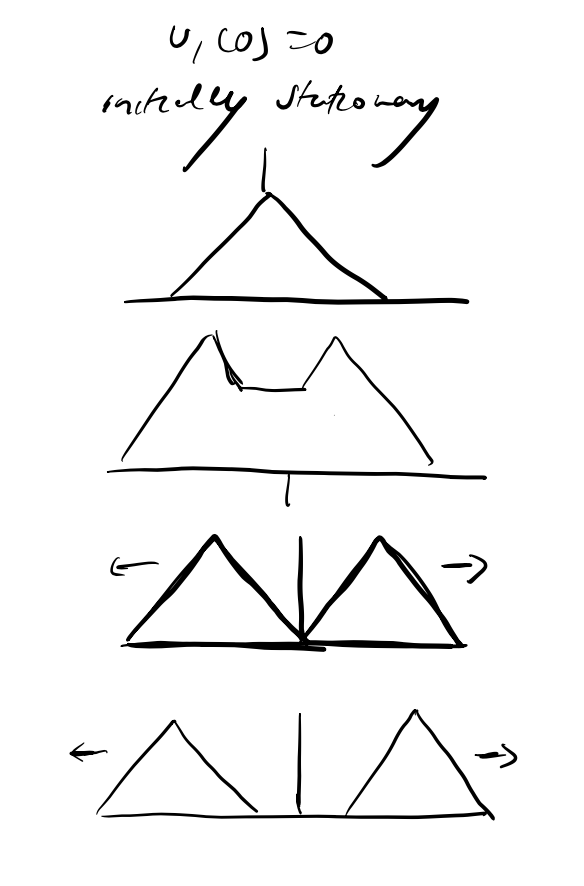
\includegraphics[width=0.45\textwidth]{waveevolution1.png} % jpg/png/pdf/eps
\end{figure}
For no initial condition but an initial velocity that is uniform in both directions we get
\begin{figure}[H]
	\centering
	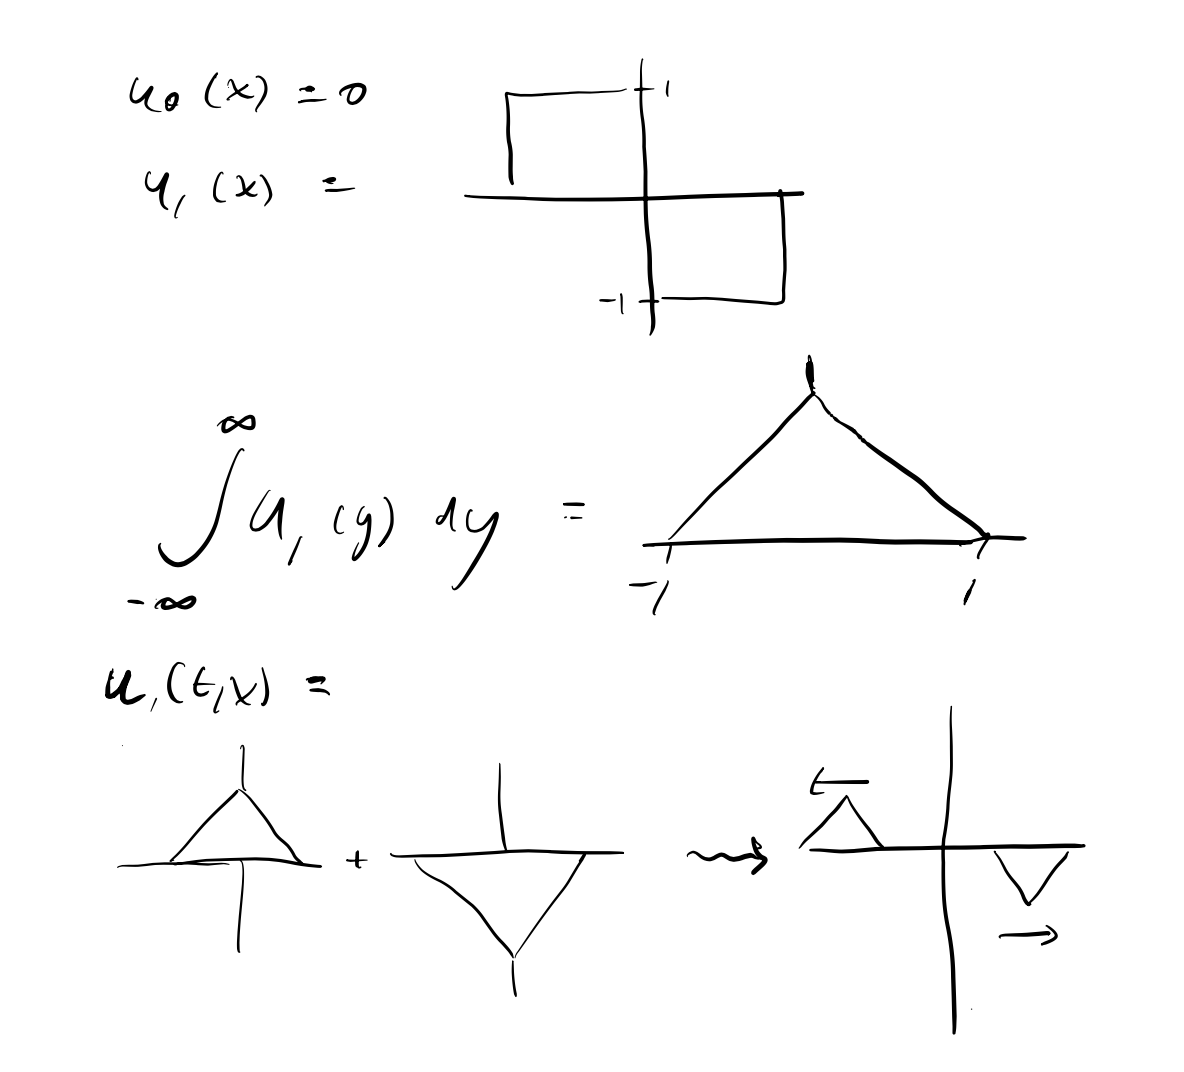
\includegraphics[width=0.65\textwidth]{waveevolution2.png} % jpg/png/pdf/eps
\end{figure}
 Now we will include a nontrivial $f(t,x)$
\begin{itemize}
\item $u_{tt}-u_{xx} = f(t,x)$
\item $u(0,x) = u_{0}(x)$
\item$u_{t}(0,x) = u_{1}(x)$
\end{itemize}
Because the operator as linear we can treat it as 3 different problems and take the sum of solutions to get the complete solution. First solution is
\begin{itemize}
	\item $u^{(1)}_{tt}-u^{(1)}_{xx} = f(t,x)$
	\item $u^{(1)}_{0}(x) = 0$
	\item$ u^{(1)}_{1}(x) = 0$
\end{itemize}
Second solution is
\begin{itemize}
	\item $u^{(2)}_{tt}-u^{(2)}_{xx} = 0$
	\item $u^{(2)}_{0}(x) = u_{0}(x)$
	\item$ u^{(2)}_{1}(x) = 0$
\end{itemize}
Third solution is
\begin{itemize}
	\item $u^{(3)}_{tt}-u^{(3)}_{xx} = 0$
	\item $u^{(3)}_{0}(x) = 0$
	\item$ u^{(3)}_{1}(x) = u_{1}(x)$
\end{itemize}
So
$$
u(t,x) = u^{(1)}(t,x) + u^{(2)}(t,x) + u^{(3)}(t,x)
$$
We already have the solution to the (2) and (3). Using the coordinates from earlier we have
$$
u_{\eta\xi} = -\frac{1}{4}f(\frac{\xi - \eta}{2},\frac{\xi + \eta}{2}) \Rightarrow u_{\xi} = C(\xi) - \int_{\eta_{0}(\xi)}^{\eta}\frac{1}{4}f(\frac{\xi - \eta^{\prime}}{2},\frac{\xi + \eta^{\prime}}{2})d\eta^{\prime}\Rightarrow
$$
$$
u(\eta,\xi) = C(\xi)+C(\eta) - \frac{1}{4}\int_{\xi_{0}}^{\xi}d\xi\int_{\eta_{0}}^{\eta}\frac{1}{4}f(\frac{\xi^{\prime} - \eta^{\prime}}{2},\frac{\xi^{\prime} + \eta^{\prime}}{2})d\eta^{\prime}
$$
\begin{center}
\textcolor{red}{Derive domain of integration, why are the constants 0}
\end{center}
Now we have
$$
u(\eta,\xi)=   \frac{1}{4}\int_{-\infty}^{\xi}d\xi\int_{\eta}^{\infty}\frac{1}{4}f(\frac{\xi^{\prime} - \eta^{\prime}}{2},\frac{\xi^{\prime} + \eta^{\prime}}{2})d\eta^{\prime}
$$
but we would like our solution in terms of original coordinates like the other two solutions.
\begin{center} \textcolor{red}{domain of integration again and change of variables}
\end{center}
$$
u^{(3)}(t,x) = \frac{1}{2}\int_{0}^{t}dt^{\prime}\int_{x-(t-t^{\prime})}^{x+(t-t^{\prime})}f(t^{\prime},x^{\prime})dx^{\prime}
$$
This expression does not carry over to higher dimensions, but gives us our general solution to the wave equation in (1+1) dimensions. 
\newline

Now we will study non-trivial boundary conditions. What is $u(t,x)$ when $x\in [0,\infty)$ with the same initial conditions $u_1$ and $u_2$. We have a couple of choices on what to do at the bondary. The first is the Dirichlett boundary condition where we fix the function at $x=0$ to a particular value. We could also allow the end to move. This is analgous to a the string tied to a ring around a pole at $x=0$. To do this we set $u_{x}(t,0) = 0$ so it cannot move in the x-direction, but still has the freedom to go up and down. We could even mix the boundary conditions for a more complicated problem, but these conditions occur infrequently in physical problems.
\newline

We can now apply a boundary condition to the general solution $u(x,t) = F(x+t)+G(x-t)$. 
$$
u(0,t) = 0 \Rightarrow F(t)+G(-t) = 0 \Rightarrow G(-t) = -F(t)
$$
This functional dependence suggest we use the method of reflections, similar to the method of images in electrostatics. We solve on the whole line with odd extensions of the initial data so that the boundary condition is built in. We originally had
\begin{itemize}
\item $u(0,x) =  u_{0}(x),\quad x\geq 0 $
\item $u_{t}(0,x) = u_{1}(x),\quad x\geq 0$
\end{itemize}
So we extend in the following way $u_{0}(-x) = -u_{0}(x)$ and $u_{1}(-x) = -u_{1}(x)$ when we let $x\in\mathbb{R}$. This is the same antisymmetry we have for the general solution on our restricted domain. So we can just use the solution on the whole domain with the new boundary conditions and then restrict that solution to $[0,\infty)$ to give us the solution we were originally looking for. Notice that $ u(t,-x)= -u(t,x)$ also satisfies our Dirichlett boundary condition.
	\lecture{4}{Wave Equation General Solution on a Manifold and more Boundary Conditions }
We take a detour from the main part of the course and study the $(1+1)$ wave equation with a general metric.
$$\sum_{i,j = 1}^{2}\frac{\partial}{\partial x^{i}}(a^{ij}(x^1,x^2)\frac{\partial u}{\partial x^{j}})=0, \quad \det{a^{ij}}<0$$
The metric is defined on a pseudoriemannian manifold $M$
$$
\sum_{i,j}g_{ij}(x^{1},x^{2})dx^{i}\otimes dx^{j}\in T^{*}M\otimes T^{*}M
$$
where $T^{*}M$ is the cotangent bundle of the manifold. These covectors are dual to the basis in our cotangent bundle
$$
dx^{i}(\frac{\partial}{\partial x^{j}}) = \delta^{i}_{\ j}
$$
and we have the inverse metric
$$
(g_{ij})^{-1} g^{ij} = \sum_{i,j}g^{ij}\frac{\partial}{\partial x^{i}}\otimes\frac{\partial}{\partial x^{j}} \in TM \otimes TM
$$
where $TM$ is the tangent bundle. It is easy to show that this is in fact the inverse of $g_{ij}$. We can use this to construct the general laplacian on a manifold (Laplace-Beltrami Operator)
\begin{align}
	\Delta_{g} u 
	= \frac{1}{\sqrt{|\det g|}}
	\sum_{i,j}
	\frac{\partial}{\partial x^{i}}
	\!\left(
	\sqrt{|\det g|}\, g^{ij}
	\frac{\partial u}{\partial x^{j}}
	\right).
\end{align}
It follows that in our wave equation
$$
a^{ij} = \sqrt{|\det{g}|}g^{ij}
$$
To simplify the form of this equation we would like to find a change of coordinates that such that $g_{ij}dx^{i}dx^{j}\to 2f(\xi,\eta)d\xi d\eta$ like the simpification we did at the beginning of lecture 3 in Euclidean space. This allowed us to find the general solution in terms of specified initial conditions. If this is the case the metric will have the form
$$
g_{ij} = 
\begin{pmatrix}
	0 & f\\
	f & 0
\end{pmatrix}, \quad \sqrt{|\det{g}|} = f \Rightarrow a^{ij} = \begin{pmatrix}
0 & 1\\
1& 0
\end{pmatrix}
$$
So our wave equation on a manifold simplifies to 
$$ \frac{1}{f}\partial_{\xi}\partial_{\eta} u = 0$$
Let us try to understand why this works. First consider the metric acting on a vector and try to solve for the vectors that are annhilated by it.
$$
\sum_{i,j}g_{ij}dx^{i}dx^{j}(\sum_{k}v^{k}\frac{\partial}{\partial x^{k}}) = \sum_{i,j}g_{ij}v^{i}v^{j} = 0 \Leftrightarrow (v^{1})^{2}-(v^{2})^{2} = 0
$$
Integrating these vectors along a path describes light-like geodesics like General Relativity. \begin{figure}[H]
	\centering
	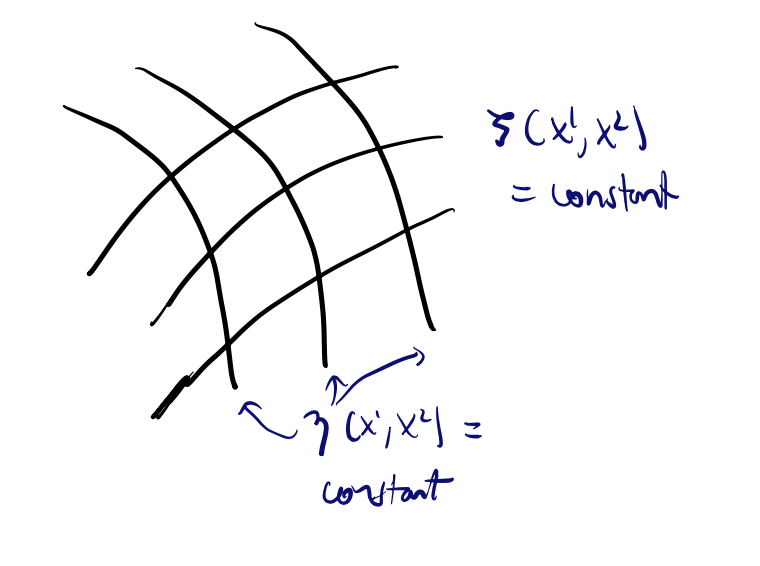
\includegraphics[width=0.65\textwidth]{desiredcoordinates.png} % jpg/png/pdf/eps
\end{figure}
$\xi$ and $\eta$ are our preferred coordinates that simplify the metric. The metric is 0 along the curves. Let us consider an example metric where we find the desired change of coordinates. There is an example in the video from minutes 31-58. But its a bit above the scope of this class, so we leave it out.
Now we return to the boundary conditions we were studying at the end of lecture 3. 
\begin{figure}[H]
	\centering
	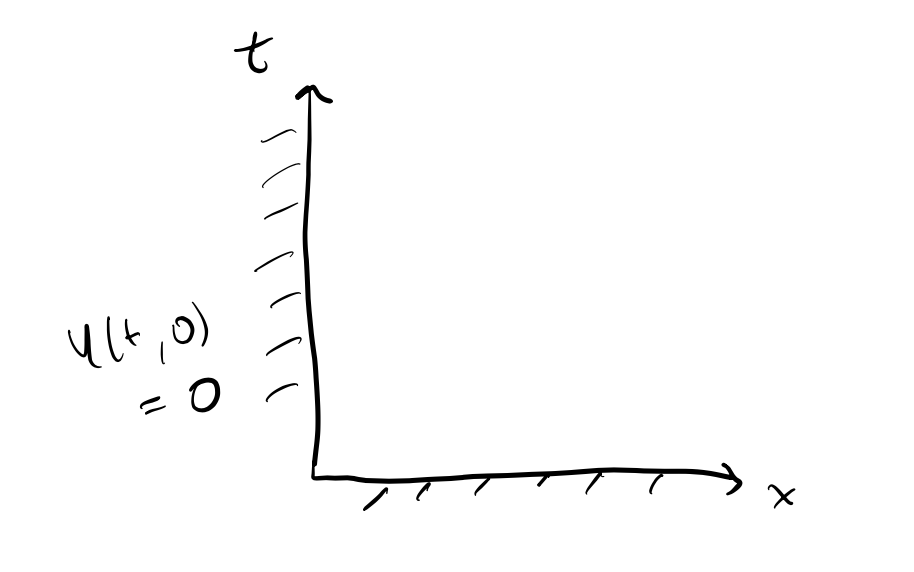
\includegraphics[width=0.4\textwidth]{dirichlett.png} % jpg/png/pdf/eps
\end{figure}
and set $u(t,0)=0$, the Dirichlett boundary condition. To find the solution to this restricted domain, we extend the solution to all of $\mathbb{R}$ by
$$
u(t,x) = -u(t,-x)
$$
We now have a mirror image on the opposite side of our boundary at $x=0$.
\begin{figure}[H]
	\centering
	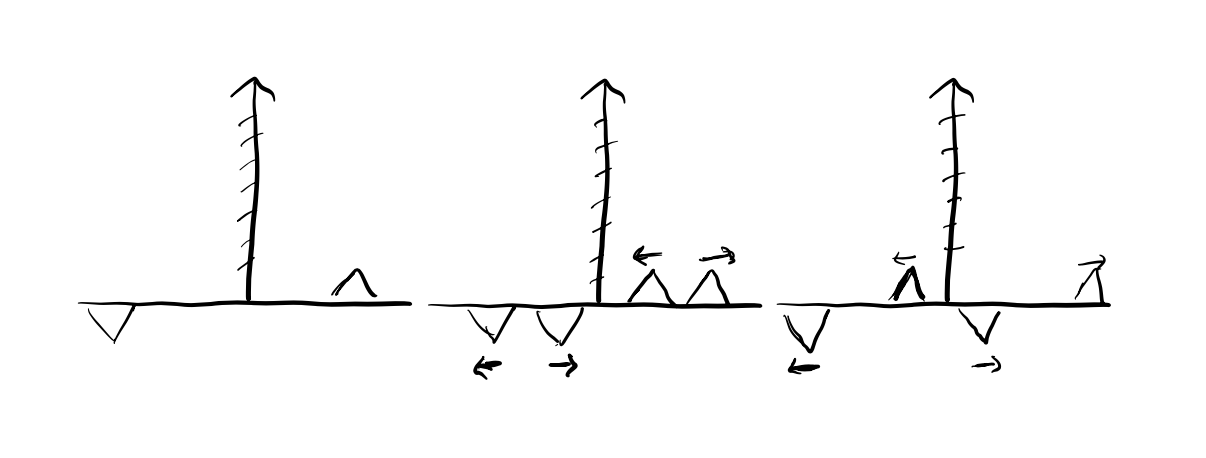
\includegraphics[width=0.6\textwidth]{reflection.png} % jpg/png/pdf/eps
\end{figure}
We now consider the Von Neumann boundary condition. Similar to the image above, we set $u_{x}(t,0) = 0$ and extend with 
$$
u(t,-x) = u(t,x)
$$
Taking the derivatives of both side of this extension equation we can see that the extension agrees at the boundary with our solution on the restricted domain. Now we have solutions like
\begin{figure}[H]
	\centering
	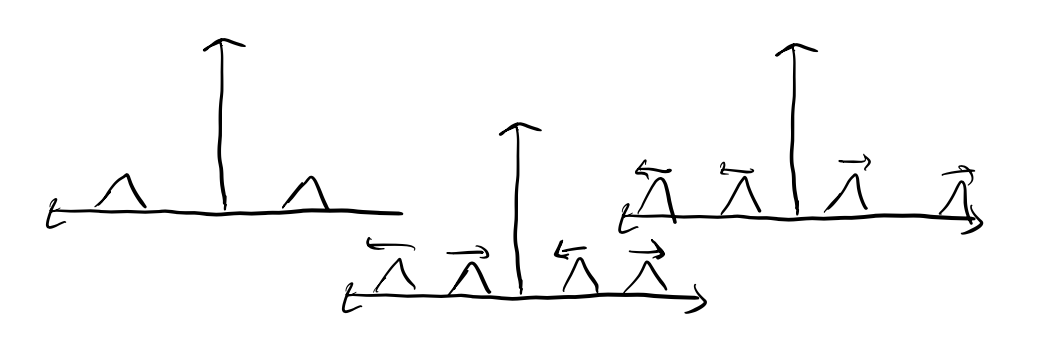
\includegraphics[width=0.6\textwidth]{vn.png} % jpg/png/pdf/eps
\end{figure}
Another interesting case are periodic and antiperiodic boundary conditions. These are described on a periodic system by $u(t,x+L)= \pm u(t,x)$. 
\begin{figure}[H]
	\centering
	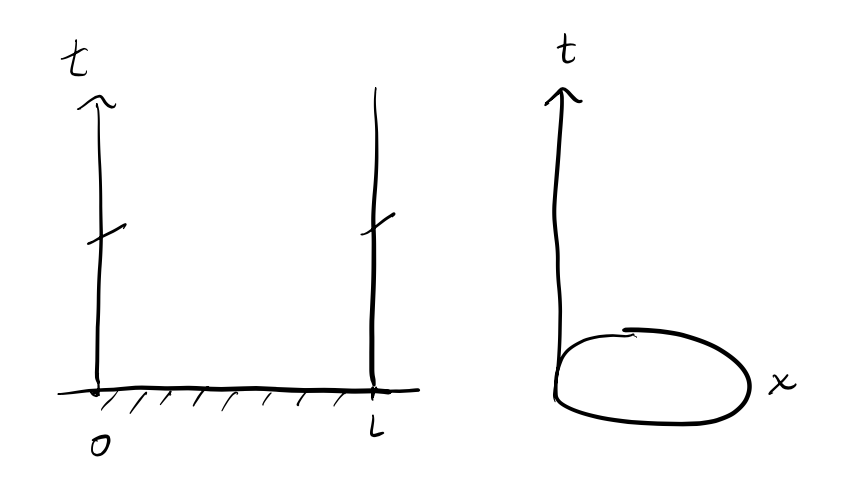
\includegraphics[width=0.6\textwidth]{pbc.png} % jpg/png/pdf/eps
\end{figure}

We start with antiperiodic solutions because we can use them to build periodic solutions by doubling the interval. Recall $u(x,t) = F(x+t)+G(x-t)$. with initial conditions $F(x)+G(x) = u_{0}(x)$ and $F^{\prime}(x)-G^{\prime}(x)= u_{1}(x)$. These conditions are on $x\in[0,L]$ but we can extend them with our periodic conditions $u_{0}(x+L) = u_{0}(x)$ and $u_{1}(x+L) = u_{1}(x)$

\problems{
\begin{exercise}
	Check that the general solution of the equation
	\[
	\partial_x\!\left( \frac{xy}{x^2 + y^2} \, \partial_x u \right)
	+ \frac{1}{2}\partial_x\!\left( \frac{x^2 - y^2}{x^2 + y^2} \, \partial_y u \right)
	+ \frac{1}{2}\partial_y\!\left( \frac{x^2 - y^2}{x^2 + y^2} \, \partial_x u \right)
	- \partial_y\!\left( \frac{xy}{x^2 + y^2} \, \partial_y u \right) = 0
	\]
	is given by
	\[
	u(x, y) = F(x^2 - y^2) + G(xy).
	\]
\end{exercise}
\solution{
Let us define
$$
\xi = x^{2}-y^{2},\quad \eta = xy
$$
which gives us 
$$
\partial_{x} = y\partial_{\eta}+2x\partial_{\xi},\quad \partial_{y} = x\partial_{\eta}-2y\partial_{\xi}
$$
We want our equation completely in terms of $\eta$ and $\xi$ so we must find $x(\xi,\eta)$ and $y(\xi,\eta)$.
Let us solve the system
\begin{itemize}
\item $(y\partial_{\eta}+2x\partial_{\xi}) x = 1$
\item $(y\partial_{\eta}+2x\partial_{\xi})y = 0$
\item $(x\partial_{\eta}-2y\partial_{\xi}) y = 1$
\item $(x\partial_{\eta}-2y\partial_{\xi}) x = 0$
\end{itemize}
\textcolor{red}{I don't know how to solve these.} Alternatively we can use the definitions to derive
$$
-x^{4}+\xi x^{2}+\eta^{2} = 0, \quad y^{4}+\xi y^{2} - \eta^{2}
$$
to get
$$
x^{2} = \frac{\xi\mp\sqrt{\xi^{2}+4\eta}}{2},\quad y^{2} = \frac{-\xi\pm\sqrt{\xi^{2}+4\eta^{2}}}{2}
$$
}
\begin{exercise}
	Solve the wave equation:
	\[
	u_{tt} - u_{xx} = f(t, x), \quad u(0, x) = u_t(0, x) = 0,
	\]
	where
	\[
	f(t, x) = (\theta_H(t - 1) - \theta_H(t - 3)) \, (\theta_H(x + 1) - \theta_H(x - 1)).
	\]
\end{exercise}
\solution{We are solving on $\mathbb{R}$ with two specified initial conditions and and driving function $f(t,x)$. We use the linearity of the equation to solve it in pieces. For the homogenous piece we have 
\begin{itemize}
\item $u^{\text{free}}_{tt} - u^{\text{free}}_{xx} = 0$
\item $u_{0}(x) = 0$
\item $u_{1}(0)=0$
\end{itemize}
We see that the free solution is trivial
$$
u^{\text{free}}(t,x) = \frac{1}{2}\big[u_{0}(x+t)+u_{0}(x-t)+ \int_{x-t}^{t+x}u_{1}(y)dy\big]
=0$$
}
Now we solve for the driven part
$$
u^{\text{driven}}(t,x) = \frac{1}{2}\int_{0}^{t}dt^{\prime}\int_{x-(t-t^{\prime})}^{x+(t-t^{\prime})}f(t^{\prime},x^{\prime})dx^{\prime}
$$
We have four integrals of the form
$$
\frac{1}{2}\int_{0}^{t}\Theta_{H}(t^{\prime}-i)dt^{\prime}\int_{x-(t-t^{\prime})}^{x+(t-t^{\prime})}\Theta_{H}(x^{\prime}-j)dx^{\prime}
$$
\textcolor{red}{Ask for help}

\begin{exercise}
	Solve the wave equation in $\mathbb{R}^{1+1}$:
	\[
	u_{tt} - u_{xx} = \theta_H(x + 3) - 2\theta_H(x + 2) + 2\theta_H(x - 2) - \theta_H(x - 3),
	\quad u(0, x) = u_t(0, x) = 0.
	\]
	You may first consider the case $t > 4$, and then obtain the solution for arbitrary $t$.
\end{exercise}
\solution{
The driving is constant in time, but varies across the spatial domain.
\newline
\textcolor{red}{Ask for help}

}
\begin{exercise}
	Solve the wave equation $u_{tt} - u_{xx} = 0$ on $\mathbb{R}$ with the following initial conditions:
	\[
	u_t(0, x) = |1 - x^2|\theta_H(1 - x^2), \qquad u(0, x) = 0,
	\]
	where $\theta_H(x) = 0$ for $x \le 0$ and $\theta_H(x) = 1$ for $x > 0$.  
	Plot this solution for some values of $t$.
\end{exercise}
\solution{
Now we use the free solution in terms of the initial conditions
$$
u^{\text{free}}(t,x) = \frac{1}{2}\big[u_{0}(x+t)+u_{0}(x-t)+ \int_{x-t}^{t+x}u_{1}(y)dy\big]
=0$$
}



\begin{exercise}
	Solve the equation
	\[
	u_{tt} - 2u_{xx} - u_{tx} = 0, \quad u_t(0, x) = 0, \quad u(0, x) = (1 - x^2)\theta_H(1 - x^2).
	\]
\end{exercise}


}
\lecture{5}{End of wave equation boundary problems (time dependent) and General Strategies for PDEs (Greens Function)}
To finish off boundary conditions for the wave equation, let us consider time dependent boundary conditions for
$$
u_{tt}-u_{xx}=0
$$
We have the same initial conditions supplied but now a constraint at the boundary
\begin{figure}[H]
	\centering
	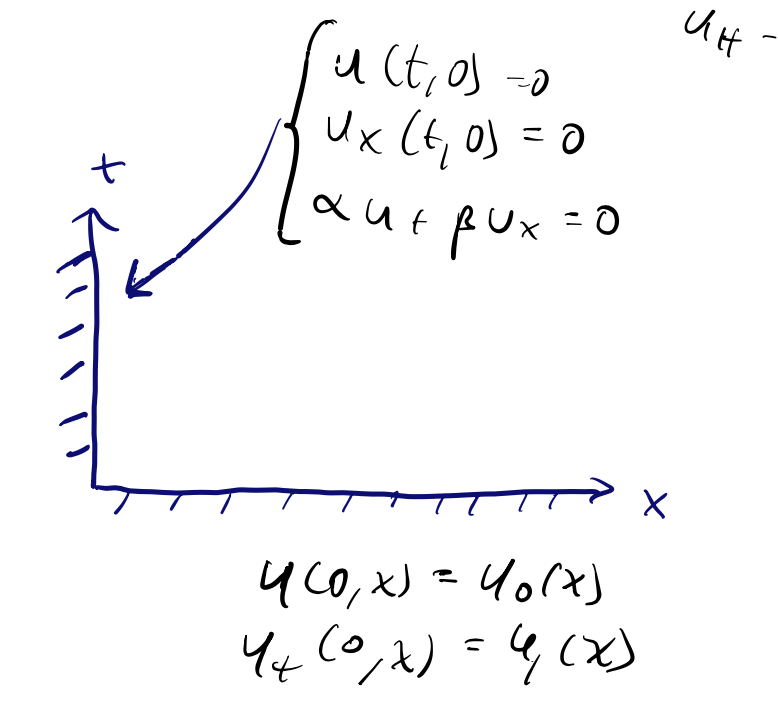
\includegraphics[width=0.65\textwidth]{time1.png} % jpg/png/pdf/eps
\end{figure}
We could even consider two boundaries
\begin{figure}[H]
	\centering
	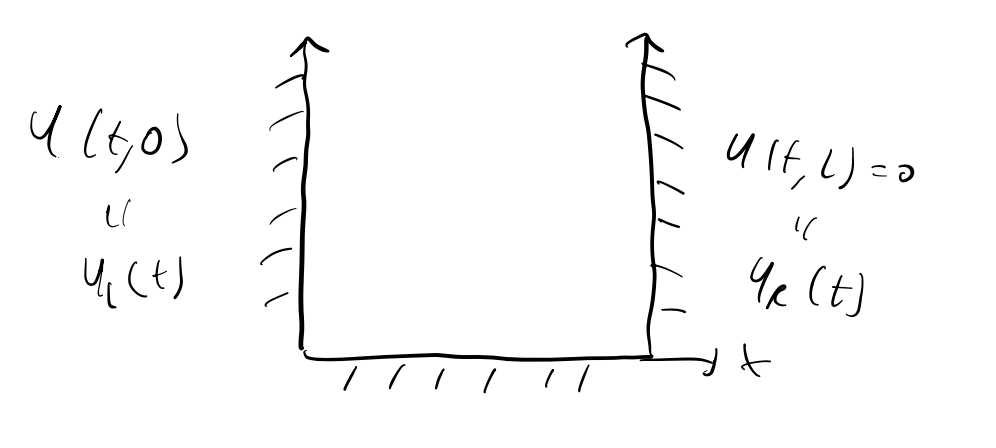
\includegraphics[width=0.65\textwidth]{time2.png} % jpg/png/pdf/eps
\end{figure}
The strategy is to try and reduce it to a problem we know how to solve. We can transfer the boundary conditions to the right hand side by defining
$$
\tilde{u}(t,x) = u(t,x)-\frac{x}{L}u_{R}(t)-(1-\frac{x}{L})u_{L}(t)
$$
One can easily check that 
$$
\tilde{u}(t,0)-\tilde{u}(t,L)=0
$$
Now our wave equation with the new function becomes
$$
\tilde{u}_{tt}-\tilde{u}_{xx} = (u_{tt}-u_{xx})-\frac{x}{L}u^{\prime\prime}_{R}(t)-(1-\frac{x}{L})u^{\prime\prime}_{L}(t) = -\frac{x}{L}u^{\prime\prime}_{R}(t)-(1-\frac{x}{L})u^{\prime\prime}_{L}(t)
$$
\textcolor{red}{I don't understand this strategy} The second strategy is to use our known solution on the real line and match it to the boundary condition, so when we restrict the domain it give us the solution we desire.
\begin{figure}[H]
	\centering
	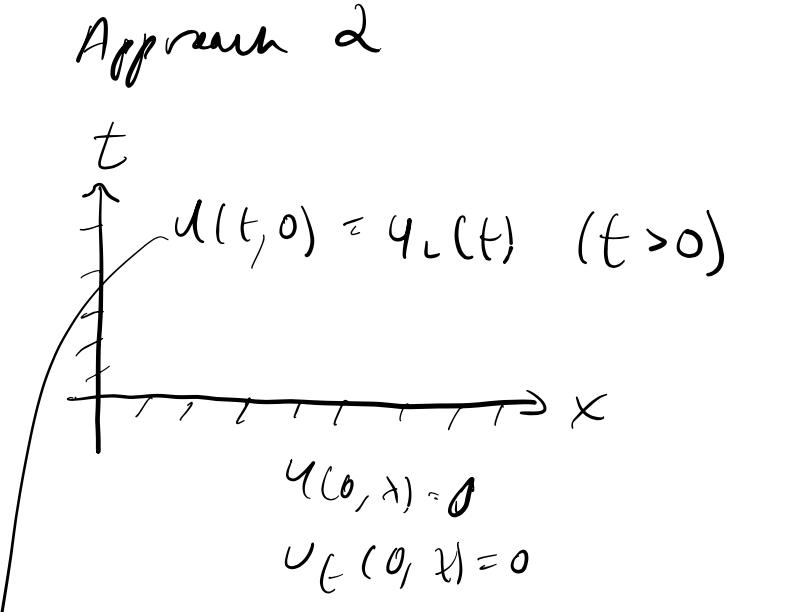
\includegraphics[width=0.65\textwidth]{Approach2.png} % jpg/png/pdf/eps
\end{figure}
Recall the general solution on the real line had the form
$$
u(t,x) =  F(t-x)+G(t+x)
$$
We can now define this for $u_{L}(t)=0$ for $t<0$. The wave will enter from the left and always match our boundary condition. We notice that taking spatial derivatives of our general form flips the sign. 
\textcolor{red}{fill in the rest of this derivation from video}
$$
u(t,x) = u_{L}(t-x)
$$
\begin{itemize}
\item solution to our wave equation
\item $u(t,0) = u_{L}(t)$
\item $u(t=0,x) = u(0,x) = u_{L}(-x), x>0$
\item$u_{t}(0,x) = u_{L}^{\prime}(-x)$
\end{itemize}
\begin{figure}[H]
	\centering
	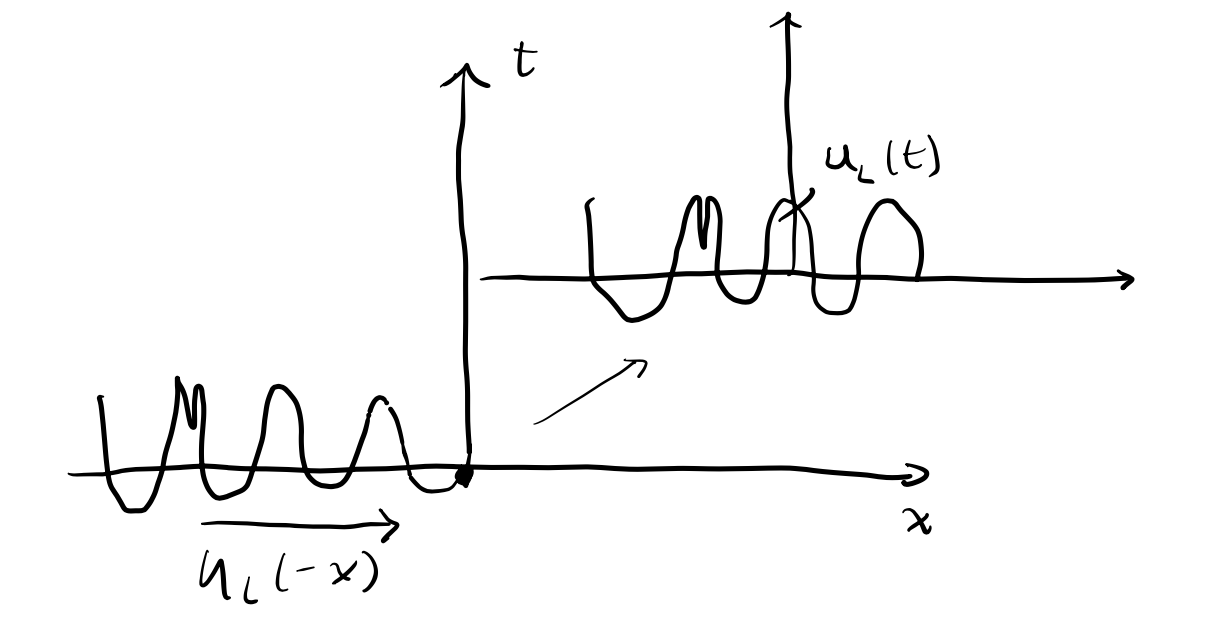
\includegraphics[width=0.65\textwidth]{fromLeft.png} % jpg/png/pdf/eps
\end{figure}
This ends our discussion on the $(1+1)$ wave equation. Now we transition to general strategies for solving PDEs.
The three main stratgeies are
\begin{enumerate}
\item Just solve it like we have done with the wave equation by integrating
\item Find a Green's function to undo the operator
\item Fourier Transform to get a more easily solvable form
\end{enumerate}
In $(1+1)$ dimensions for a driven wave on $\mathbb{R}$ we had 
$$
u(t,x) = \frac{1}{2}\int_{0}^{t}dt^{\prime}\int_{x-|t-t^{\prime}|}^{x+|t-t^{\prime}|}dx^{\prime}f(t^{\prime},x^{\prime})
$$
We expect this to generalize to $1+d$ with
$$
u(t,\vec{x})= \frac{1}{2}\int_{\mathbb{R}^{d+1}}dt^{\prime}d\vec{x}^{\prime}G(t,\vec{x};t^{\prime},\vec{x}^{\prime}) f(t^{\prime},\vec{x}^{\prime})
$$
We can read off the explicit form of the green's function from the integral solution. Recall the the Heaviside function $\theta_{H}(x)$ is defined as
\[
\theta_H(x) =
\begin{cases}
	0, & x < 0, \\
	\frac{1}{2}, & x = 0, \\
	1, & x > 0.
\end{cases}
\]
For $d+1$ we have
$$
G(t,x;t^{\prime},x^{\prime}) = \frac{1}{2}\theta_{H}(t-t^{\prime})\theta_{H}(t^{\prime})[\theta_{H}(x-x^{\prime}+|t-t^{\prime}|)-\theta_{H}(x-x^{\prime}-|t-t^{\prime}|)]
$$
\textcolor{red}{Exercise: check that this is describing the function over the domain of integration} This shows us that our Green's functio approach matches our integration approach. To understand the Green's function better let us study the discretization of 
$$
u_{tt}-\Delta u +\alpha u = f
$$
on a periodic boundary.
\begin{figure}[H]
	\centering
	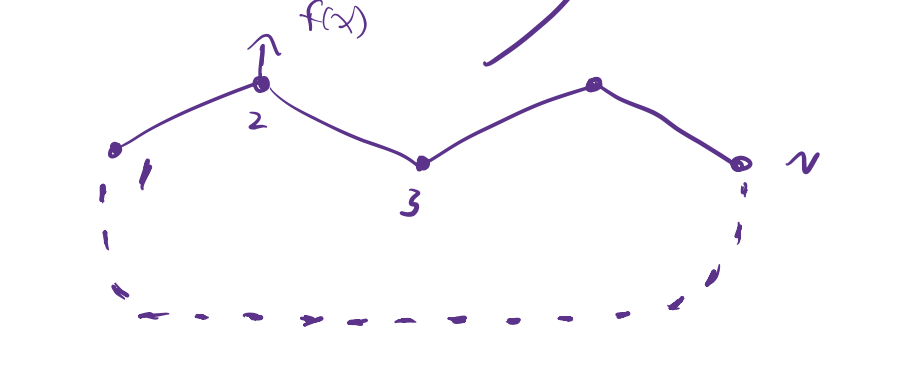
\includegraphics[width=0.65\textwidth]{periodicchain.png} % jpg/png/pdf/eps
\end{figure}
We identify $f(N+1)\sim f(1)$. The discrete version of this equation is
$$
-u(t,x+1)+ 2u(t,x)-u(t,x-1)+\alpha u(t,x) = f(x)
$$
Neglecting time dependence will simplify the problem. So we are solving for a stationary state.
For $x\in\{1,...,N\}$ we have
$$
-u(x+1) + 2u(x)-u(x-1)+\alpha u(x) = f(x)
$$
If we have $\vec{u}=[u(1),...,u(N)]^{T}$ and $\vec{f} = [f(1),...,f(N)]^{T}$ then the corresponding matrix is
\[
A =
\begin{pmatrix}
	2+\alpha & -1        & 0         & \cdots  & 0         & -1 \\
	-1        & 2+\alpha & -1        & \cdots  & 0         & 0  \\
	0         & -1        & 2+\alpha & \ddots  & \vdots    & \vdots \\
	\vdots    & \ddots   & \ddots    & \ddots  & -1        & 0 \\
	0         & 0         & \cdots   & -1      & 2+\alpha  & -1 \\
	-1        & 0         & \cdots   & 0       & -1        & 2+\alpha
\end{pmatrix}
\]
for the equation $T\vec{u} = \vec{f}$. So $T\sim \tilde{\alpha}-\tilde{\Delta}$. The solution for $\vec{u}$ is found by inverting this matrix. This is the greens function for a finite dimensional system.
$$
\vec{u} = (\alpha-\Delta)^{-1}\vec{f}=G\vec{f}
$$
We can express $G$ as a matrix
\[
G =
\begin{pmatrix}
	G(1,1) & G(1,2) & G(1,3) & \cdots & G(1,N) \\
	G(2,1) & G(2,2) & G(2,3) & \cdots & G(2,N) \\
	G(3,1) & G(3,2) & G(3,3) & \cdots & G(3,N) \\
	\vdots & \vdots & \vdots & \ddots & \vdots \\
	G(N,1) & G(N,2) & G(N,3) & \cdots & G(N,N)
\end{pmatrix}
\]
This gives us
$$
u(x)=\sum_{x^{\prime}}^{N}G(x,x^{\prime})f(x^{\prime})$$
we compare this with the earlier solution
$$
\vec{u}(t,\vec{x})= \frac{1}{2}\int_{\mathbb{R}^{d+1}}dt^{\prime}d\vec{x}^{\prime}G(t,\vec{x};t^{\prime},\vec{x}^{\prime}) f(t^{\prime},\vec{x}^{\prime})
$$ 
and note the similarities
\begin{enumerate}
\item $x^{\prime}\leftrightarrow(t^{\prime},\vec{x}^{\prime})$	
\item $\sum_{x^{\prime}}\leftrightarrow \int dt^{\prime}d\vec{x}^{\prime}$
\item $G(x,x^{\prime})\leftrightarrow G(t,x;t^{\prime},x^{\prime})$
\end{enumerate}
The equation satisfied by the greens function is 
$$
(\alpha-\Delta)\cdot G = \mathbb{I} \Leftrightarrow [(\alpha-\Delta)\cdot G](x,x^{\prime}) = \delta_{x,x^{\prime}}
$$
For a particular $x_{0}$ we have
$$
-G(x_{0}+1,x^{\prime})+(\alpha+2)G(x_{0},x^{\prime})-G(x_{0}-1,x^{\prime})= \delta_{x_{0},x^{\prime}}
$$
We see this is exactly the same equation as earlier but $f(x)$ has been replaced by a delta function. This is drastically simpler. Now we have $f(x_{0}) = [0,...,1,....,0]^{T}$ with 1 at the $x_{0}^{\text{th}}$ position
We can expand out $f(x)$ by
$$
f(x) = \sum_{x^{\prime}}^{N}\delta_{x,x^{\prime}}f(x^{\prime})
$$
Using linearity we have

\begin{align*}
	(\alpha I - \Delta_x)\,u(x)
	&= (\alpha I - \Delta_x)\sum_{x'=1}^N G(x,x')\,f(x') \\
	&= \sum_{x'=1}^N \bigl[(\alpha I - \Delta_x)G(x,x')\bigr]\,f(x') \\
	&= \sum_{x'=1}^N \delta_{x,x'}\,f(x') \\
	&= f(x).
\end{align*}
We see that the Green's function is the inverse of the operator satisfies a much simpler equation 
$$
(\alpha - \Delta_{x})G(x,x^{\prime})=\delta_{x,x^{\prime}}
$$
or 
$$
(\partial_{t}^{2}-\Delta)G(t,\vec{x};t^{\prime},x^{\prime}) = \delta(t-t^{\prime})\delta^{(d)}(\vec{x}-\vec{x}^{\prime})
$$
The Greens function has the same form in the discrete case and the continuous case.
\textcolor{red}{End of Lecture we start to study Fourier Transforms}





\newpage
\problems{
	\begin{exercise}
		Solve the wave equation on a half-line $x > 0$:
		\[
		u_{tt} - u_{xx} = 0, \quad u(0, x) = 0, \quad u_t(0, x) = \theta_H(x - 3) - \theta_H(x - 2), \quad u(t, 0) = 0.
		\]
		For simplicity, consider only the large time case.
	\end{exercise}
	\begin{exercise}
		Solve the wave equation $u_{tt} - u_{xx} = 0$ on $\mathbb{R}_{>0}$ with the following initial and boundary conditions:
		\[
		u_t(0, x) = 0, \quad u(0, x) = \sin^2(2\pi x)\theta_H(1 - |x - 2|), \quad
		u(t, 0) = \tfrac{1}{2}\sin^2(2\pi t)\theta_H(1 - |t - 2|).
		\]
		Plot this solution for some values of $t$.
	\end{exercise}
	\begin{exercise}
		Solve the wave equation on a half-line $x > 0$:
		\[
		u_{tt} - u_{xx} = \theta_H(1 - x), \quad u(0, x) = 0, \quad u_t(0, x) = 0, \quad u(t, 0) = 0,
		\]
		where $\theta_H$ is the Heaviside theta function:
		\[
		\theta_H(x) =
		\begin{cases}
			0, & x < 0, \\
			1, & x > 0, \\
			\frac{1}{2}, & x = 0.
		\end{cases}
		\]
		For simplicity, consider its solution only for $t > 4$.
	\end{exercise}
\begin{exercise}
	Find the Green function of the discrete Laplace operator on a finite lattice with periodic boundary conditions $(\mathbb{Z}/N\mathbb{Z})$, $\Delta = T + T^{-1} - 2$.  
	Solve this problem directly, then check that the obtained result is consistent with the Fourier transform.
\end{exercise}
\begin{exercise}
	Solve the following initial and boundary value problems on the rectangle $x \in [0, L]$, $t \in [0, T]$, with zero boundary conditions $u(t, 0) = u(t, L) = 0$:
	\[
	\begin{cases}
		u_{tt}(t, x) - u_{xx}(t, x) = 0, & u(0, x) = \sin^3 \frac{\pi x}{L}, \; u_t(0, x) = \sin \frac{2\pi x}{L}, \\
		u_{tt}(t, x) + u_{xx}(t, x) = 0, & u(0, x) = \sin \frac{\pi x}{L}, \; u(T, x) = \sin^3 \frac{\pi x}{L}.
	\end{cases}
	\]
\end{exercise}
\begin{exercise}
	Find explicitly the Green function of the operator $\Delta - m^2$ in the 5-dimensional space.
	
	Hint: try to use an ansatz
	\[
	G(r) = \frac{e^{-mr}P(mr)}{r^3}
	\]
	with some polynomial $P$.
\end{exercise}

}
\lecture{6}{General Strategies Continued (Fourier Transform)}
\problems{
\begin{exercise}
	Study the Fourier transform on a segment $x = 1, \dots, N$:
	\begin{enumerate}
		\item Compute scalar products between the functions $\varphi_k(x) = \sin\frac{\pi kx}{N+1}$, $k = 1, \dots, N$:
		\[
		(\varphi_k, \varphi_{k'}) = \sum_{x=1}^{N} \varphi_k(x)\varphi_{k'}(x).
		\]
		\item Write the formulas for the direct and inverse Fourier transform.
	\end{enumerate}
\end{exercise}


\begin{exercise}
	Compute the Fourier transforms of the following functions on a circle $\varphi \in [0, 2\pi)$:
	\[
	f_1(\varphi) = \varphi, \qquad f_2(\varphi) = |\pi - \varphi|.
	\]
	For $f_1$, determine the asymptotic behavior of the coefficients at large $n$.  
	For $f_2$, compute $f_2(0)$ and compare it with its Fourier series at this point. Does it yield any non-trivial identity?
\end{exercise}

\begin{exercise}
	Compute the Fourier transforms of the following functions on the real line:
	\[
	f_3(x) = \frac{1}{\cosh x}, \qquad f_4(x) = (1 - 2x^2)e^{-x^2/2}.
	\]
\end{exercise}

\begin{exercise}
	Define the Fourier transform for the function on a segment $x \in [0, L]$, vanishing at the boundaries, by
	\[
	f(x) = \sum_{k=1}^{\infty} \tilde{f}_k \sin\frac{\pi kx}{L}.
	\]
	Find the inverse transformation.
\end{exercise}
\begin{exercise}
	Find the Fourier transform of the function
	\[
	f(x) = \frac{1}{e^{2\pi i x} - \frac{1}{2}}
	\]
	on a circle $x \sim x + 1$.
\end{exercise}

\begin{exercise}
	Find the Fourier transform of the function
	\[
	f(x) = \frac{1}{\cos(2\pi x) - \cosh(2\pi a)}
	\]
	on a circle $x \sim x + 1$.
\end{exercise}

\begin{exercise}
	Find the Fourier transform of the function
	\[
	f(x) = \frac{1}{x^2 + 1}
	\]
	on $\mathbb{R}$.
\end{exercise}

\begin{exercise}
	Find the Fourier transform of the function
	\[
	f(x) = \frac{\sin x}{x^2 + 1}
	\]
	on $\mathbb{R}$.
\end{exercise}

\begin{exercise}
	Find the Fourier transform of the function
	\[
	f(x) = \frac{\sin x}{x}
	\]
	on $\mathbb{R}$.
\end{exercise}

}

\lecture{X}{More Problems}
\problems{

\begin{exercise}
	Solve the equation
	\[
	u''(t) + \omega^2 u(t) = f(t), \quad u(0) = u_0, \quad u'(0) = u_1.
	\]
\end{exercise}










\begin{exercise}
	Find the plane wave solution of Maxwell’s equations.
\end{exercise}


\begin{exercise}
	Compute the Fourier transform of $\operatorname{v.p.}\frac{1}{\omega}$, then check that the inverse Fourier transform recovers the initial (generalized) function.
\end{exercise}

\begin{exercise}
	Solve the following equation:
	\[
	u''(t) + \mu^2 u(t) = \theta_H(t)\sin\Omega t, \quad u(0) = u'(0) = 0.
	\]
	What is the difference between the cases $\Omega^2 \neq \mu^2$ and $\Omega^2 = \mu^2$?
\end{exercise}

\begin{exercise}
	Solve the heat equation on the real line:
	\[
	u_t(t, x) = \Delta u(t, x), \quad u(0, x) = \theta_H(x).
	\]
	How smooth is $u(t, x)$ for $t > 0$?
\end{exercise}



\begin{exercise}
	Solve Laplace’s equation $u_{z\bar{z}} = 0$ in the unit disk $|z| \le 1$ with the following boundary conditions:
	\[
	u(e^{i\varphi}) =
	\begin{cases}
		\cos \varphi, \\
		1, & \varphi \in (0, \pi),\\
		-1, & \varphi \in (\pi, 2\pi).
	\end{cases}
	\]
\end{exercise}

\begin{exercise}
	Find the Green function of the Laplace equation in the domain
	\[
	D = \{z \mid \Im z \in [0, \pi], \; \Re z \in [0, \infty)\}
	\]
	with boundary conditions $G(z, z_0) = 0$ for $z \in \partial D$ and $G(z, z_0) \to 0$ as $\Re z \to \infty$.
	
	\textit{Idea 1:} first solve in the infinite strip, then add image charge.  
	\textit{Idea 2:} use conformal map $w(z) = \cosh z$.
\end{exercise}

\begin{exercise}
	Solve Laplace’s equation $u_{z\bar{z}} = 0$ in the domain
	\[
	D = \{z \mid \Re z \ge 0, |z - 1| \le a\}
	\]
	with boundary conditions:
	\[
	u = 0, \; z \in i\mathbb{R}, \quad
	u = u_0, \; |z - 1| = a, \quad
	u \to 0 \text{ as } z \to +\infty.
	\]
\end{exercise}

\begin{exercise}
	Solve the 3D Laplace equation $\Delta u = 0$ in the domain
	\[
	D = \{(r, \theta, \varphi) \mid r > R\}
	\]
	with boundary conditions
	\[
	u(R, \theta, \varphi) = \cos^2\theta, \qquad \lim_{r \to \infty} u(r, \theta, \varphi) = 0.
	\]
\end{exercise}

\begin{exercise}
	Find all solutions of Laplace’s equation $\Delta u(x, y, z) = 0$ which are not more than quadratic in $x, y, z$.  
	Expand them in spherical harmonics.
\end{exercise}

\begin{exercise}
	Compute the scalar product between associated Legendre polynomials:
	\[
	\int_{-1}^{1} P_l^m(x) P_k^m(x)\,dx.
	\]
	Definition:
	\[
	P_l^m(x) = (-1)^m (1 - x^2)^{m/2} \frac{d^m}{dx^m} P_l(x), \quad
	P_l(x) = \frac{1}{2^l l!} \frac{d^l}{dx^l}(x^2 - 1)^l.
	\]
\end{exercise}

\begin{exercise}
	Find the Fourier expansion of the plane wave:
	\[
	e^{ikr\sin\varphi} = \sum_{n\in\mathbb{Z}} c_n(r)e^{in\varphi}.
	\]
\end{exercise}
}


\begin{exercise}
	Find the Fourier transform of $\frac{1}{\cosh x}$.
	
	\textit{Hints:}
	\begin{itemize}
		\item Consider the difference of the two integrals over $\mathbb{R}$ and over $\mathbb{R} + 2\pi i$: first compare it with the original integral, then compute by residues.
		\item Alternatively, close the contour and compute it as a sum of residues.
	\end{itemize}
\end{exercise}

\begin{exercise}
	Solve the equation
	\[
	u_{tt} - u_{xx} = f(t, x), \quad u_t(0, x) = 0, \quad u(0, x) = 0,
	\]
	where
	\[
	f(t, x) = |1 - |x|| \, \theta_H(1 - |x|)\theta_H(t(1 - t)).
	\]
	Plot this solution, e.g. for $t = 10$.
\end{exercise}



\begin{exercise}
	Solve the equation
	\[
	u_t - u_{xx} = 0, \qquad u(0, x) = \sin x.
	\]
\end{exercise}

\begin{exercise}
	Solve the equation
	\[
	u_t - u_{xx} = 0, \quad x \ge 0, \quad |u(-\infty, x)| < \infty, \; |u(t, +\infty)| < \infty, \quad u(t, 0) = \sin t.
	\]
\end{exercise}


\begin{exercise}
	Find a formula for $P^1_{f(x)}$, analogous to
	\[
	\delta(f(x)) = \sum_{f(x_n) = 0} \frac{1}{|f'(x_n)|}\delta(x - x_n).
	\]
\end{exercise}

\begin{exercise}
	Solve the equation
	\[
	u_t(t, \vec{r}) - \Delta u(t, \vec{r}) = 0, \quad \vec{r} \in \mathbb{R}^d, \quad u(0, \vec{r}) = \vec{r}\, e^{-(\vec{r} - \vec{r}_0)^2}.
	\]
\end{exercise}

\begin{exercise}
	Solve the equation
	\[
	\Delta u(x, y) = 0, \quad x^2 + y^2 \le 1, \quad u(\cos \varphi, \sin \varphi) = \sin 2\varphi.
	\]
\end{exercise}

\begin{exercise}
	Solve the equation
	\[
	\partial_t u(t, x) - u_{xx}(t, x) = \sin x \sin t, \quad u(0, x) = 0,
	\]
	in the limit $t \to \infty$.
\end{exercise}

\begin{exercise}
	Solve the equation
	\[
	\Delta u(x, y, z) = 0, \quad x^2 + y^2 + z^2 \le 1, \quad u(\sin\theta\cos\varphi, \sin\theta\sin\varphi, \cos\theta) = \cos 2\theta.
	\]
\end{exercise}

\begin{exercise}
	Solve the equation
	\[
	\Delta u(x, y) = \delta(x - x_0)\delta(y - y_0),
	\]
	in the domain $\arg(x + iy) \in (0, \pi/3)$ with boundary conditions
	\[
	u(r\cos \tfrac{\pi}{3}, r\sin \tfrac{\pi}{3}) = u(r, 0) = 0.
	\]
\end{exercise}

\begin{exercise}
	Expand each component of the vector
	\[
	(\sin\theta\cos\varphi, \sin\theta\sin\varphi, \cos\theta)P_1(\cos\theta)
	\]
	in the basis of spherical harmonics.
\end{exercise}

\begin{exercise}
	Find solutions of the Sturm–Liouville problem
	\[
	u''(x) = -\lambda u(x), \quad u(0) = 0, \quad u'(1) = 0.
	\]
	Check that the corresponding functions $u_n(x)$ form a complete system.
\end{exercise}

\begin{exercise}
	Find the radially symmetric solution of the Helmholtz equation
	\[
	\Delta u(r) + u(r) = 0,
	\]
	regular at $r = 0$, in two and three dimensions.
\end{exercise}
\begin{exercise}
	Solve the wave equation:
	\[
	\begin{cases}
		u_{tt} - u_{xx} - u_{yy} = (\theta_H(t - 1) - \theta_H(t - 2)) \delta(x)\delta(y), & u(0, x, y) = u_t(0, x, y) = 0, \\
		u_{tt} - u_{xx} - u_{yy} - u_{zz} = (\theta_H(t - 1) - \theta_H(t - 2)) \delta(x)\delta(y)\delta(z), & u(0, x, y, z) = u_t(0, x, y, z) = 0.
	\end{cases}
	\]
\end{exercise}
\begin{exercise}
	Solve the equation
	\[
	u_{tt} - u_{xx} - u_{yy} = \delta(x)\delta(y)\theta_H(t(1 - t)), \quad t > 0, \quad u(0, x, y) = u_t(0, x, y) = 0.
	\]
\end{exercise}
\begin{exercise}
	Solve the equation
	\[
	u_t - u_{xx} = 0, \qquad u(0, x) = e^{-(x - a)^2}.
	\]
\end{exercise}
\end{document}
